
\section{Alchemical Free Energy Perturbation Calculations}
\label{section:alchemy}

This feature has been contributed to NAMD by the following authors:

\begin{quote}
Surjit B. Dixit, J\'{e}r\^{o}me H\'{e}nin and Christophe Chipot   \\[0.4cm]
   {\it Equipe de dynamique des assemblages membranaires, }   \\
   {\it UMR CNRS/UHP 7565,                                }   \\
   {\it Universit� Henri Poincar�,                        }   \\
   {\it BP 239,                                           }   \\
   {\it 54506 Vand\oe uvre--l�s--Nancy cedex, France      }
\end{quote}


%\date{\small Version: \today
%\\[10.0cm]
\copyright~2001--2006, {\sc Centre National de la Recherche Scientifique}



\subsection{Introduction}


\subsubsection{Theoretical background}


A method to perform alchemical free energy perturbation (FEP)~\cite{Zwanzig1954,Beveridge1989,VanGunsteren1989,Straatsma1992,Kollman1993,Gilson1997,
Mark1998,Chipot2002g,Chipot2007} is available in NAMD. Within the
FEP framework, the free energy difference between two alternate
states, $a$ and $b$, is expressed by:


\begin{equation}
\Delta A_{a \rightarrow b} = -\frac{1}{\beta} \ \ln
                              \left\langle \exp \left\{-\beta
                                                \left[{\cal H}_b({\bf x}, {\bf p}_x) -
                                                      {\cal H}_a({\bf x}, {\bf p}_x)
                                                \right]
                                                \right\}
                                                \right\rangle_a
\label{fep}
\end{equation}


Here, $\beta^{-1} \equiv k_B T$, where $k_B$
is the Boltzmann constant, $T$ is the temperature.
${\cal H}_a({\bf x}, {\bf p}_x)$ and ${\cal H}_b({\bf x}, {\bf p}_x)$
are the Hamiltonians characteristic of states $a$ and $b$, respectively.
$\left\langle \cdots \right\rangle_a$ denotes an ensemble average over configurations
representative of the initial, reference state, $a$.


\begin{figure}[ht]
  \center{\vspace{0.4cm}
          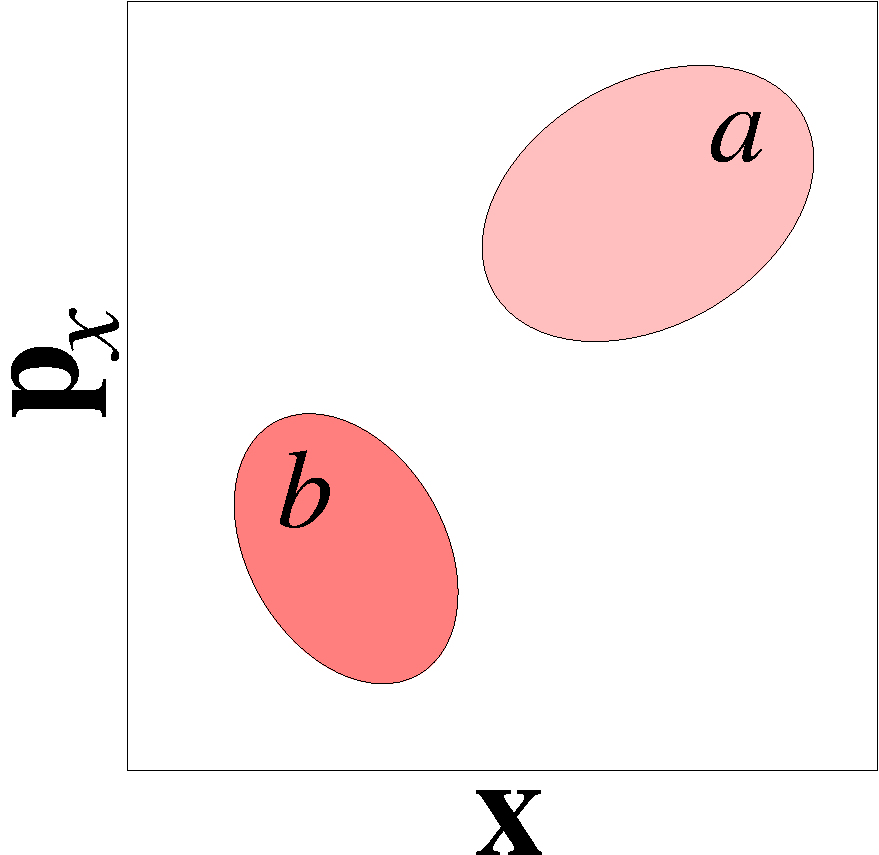
\includegraphics[width=4cm]{figures/overlap1}
          {\bfseries \sffamily (a)}
          \hfill
          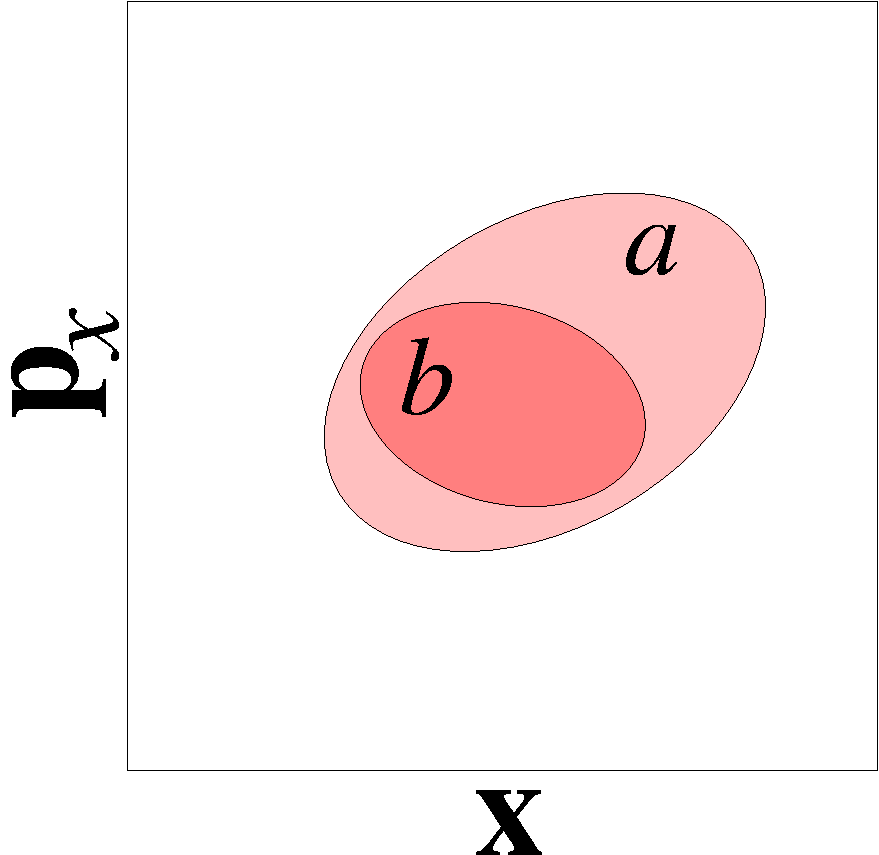
\includegraphics[width=4cm]{figures/overlap2}
          {\bfseries \sffamily (b)}
          \hfill
          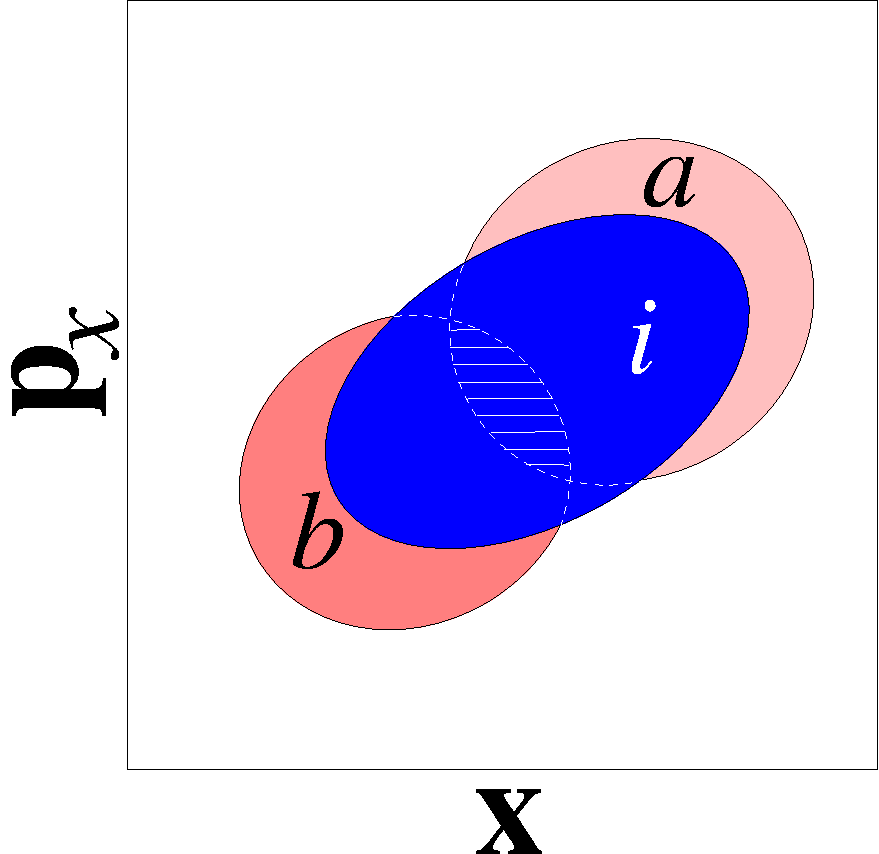
\includegraphics[width=4cm]{figures/overlap3}
          {\bfseries \sffamily (c)}}
  \caption{Convergence of an FEP calculation. If the ensembles representative
           of states $a$ and $b$ are too disparate, equation~({\ref{fep}}) will
           not converge {\bfseries \sffamily (a)}.
           If, in sharp contrast, the configurations of
           state $b$ form a subset of the ensemble of configurations
           characteristic of state $a$, the simulation is expected
           to converge {\bfseries \sffamily (b)}.
           The difficulties reflected in case {\bfseries \sffamily (a)} may be
           alleviated by the introduction of mutually overlapping intermediate
           states that connect $a$ to $b$ {\bfseries \sffamily (c)}. It should be
           mentioned that in practice, the kinetic contribution, ${\cal T}({\bf p}_x)$,
           is assumed to be identical for state $a$ and state $b$.
           \label{fig:overlap}}
\end{figure}


Convergence of equation~({\ref{fep}}) implies that low--energy
configurations of the target state, $b$, are also configurations
of the reference state, $a$, thus resulting in an appropriate overlap
of the corresponding ensembles --- see Figure~\ref{fig:overlap}.
In practice, transformation between the two thermodynamic states
is replaced by a series of transformations between non--physical,
intermediate states along a well--delineated
pathway that connects $a$ to $b$.
This pathway is characterized by a general extent parameter, often
referred to as ``coupling parameter''~\cite{Beveridge1989,Mark1998,King1993,Kirkwood1935},
$\lambda$, that makes the Hamiltonian and, hence, the free energy,
a continuous function of this parameter between $a$ and $b$:


\begin{equation}
\Delta A_{a \rightarrow b} = -\frac{1}{\beta} \ \sum_{i = 1}^N \ln
                              \left\langle \exp\left\{-\beta
                                               \left[{\cal H}({\bf x}, {\bf p}_x; \lambda_{i+1}) -
                                                     {\cal H}({\bf x}, {\bf p}_x; \lambda_i)
                                               \right]
                                               \right\}
                                               \right\rangle_i
\label{windows}
\end{equation}


Here, $N$ stands for the number of intermediate stages, or ``windows''
between the initial and the final states --- see Figure~\ref{fig:overlap}.



\subsubsection{The dual--topology paradigm}


In a typical FEP setup involving the transformation of one chemical
species into an alternate one in the course of the simulation, the atoms
in the molecular topology can be classified into three groups, (i) a
group of atoms that do not change during the simulation --- \eg the
environment, (ii) the atoms describing the reference state, $a$, of the
system, and (iii) the atoms that correspond to the target state,
$b$, at the end of the alchemical transformation. The atoms
representative of state $a$ should \emph{never} interact with those of state $b$
throughout the MD simulation. Such a setup,
in which atoms of both the initial and the final states of the
system are present in the molecular topology file --- \ie the {\tt
psf} file --- is characteristic of the so--called ``dual topology''
paradigm~\cite{Gao1989,Pearlman1994a,Axelsen1998}. The hybrid Hamiltonian of
the system, which is a function of the general extent parameter, $\lambda$,
that connects smoothly state $a$ to state $b$, is calculated as a linear
combination of the corresponding Hamiltonians:


\begin{equation}
{\cal H}({\bf x}, {\bf p}_x; \lambda)
                  = {\cal H}_0({\bf x}, {\bf p}_x)
                  + \lambda {\cal H}_b({\bf x}, {\bf p}_x)
                  + (1-\lambda) {\cal H}_a({\bf x}, {\bf p}_x)
\label{linear}
\end{equation}


where ${\cal H}_a({\bf x}, {\bf p}_x)$ describes the interaction of the group of
atoms representative of the reference state, $a$, with the rest of the system.
${\cal H}_b({\bf x}, {\bf p}_x)$ characterizes the interaction of the target topology,
$b$, with the rest of the system.
${\cal H}_0({\bf x}, {\bf p}_x)$ is the Hamiltonian describing those atoms that do not
undergo any transformation during the MD simulation.


For instance, in the point mutation of an
alanine side chain into that of glycine, by means of an FEP
calculation, the topology of
both the methyl group of alanine and the hydrogen borne by the
C$_\alpha$ in glycine co--exist throughout the simulation (see
Figure~\ref{fig:dual_top}), yet without actually seeing each
other.


\begin{figure}[ht]
  \center{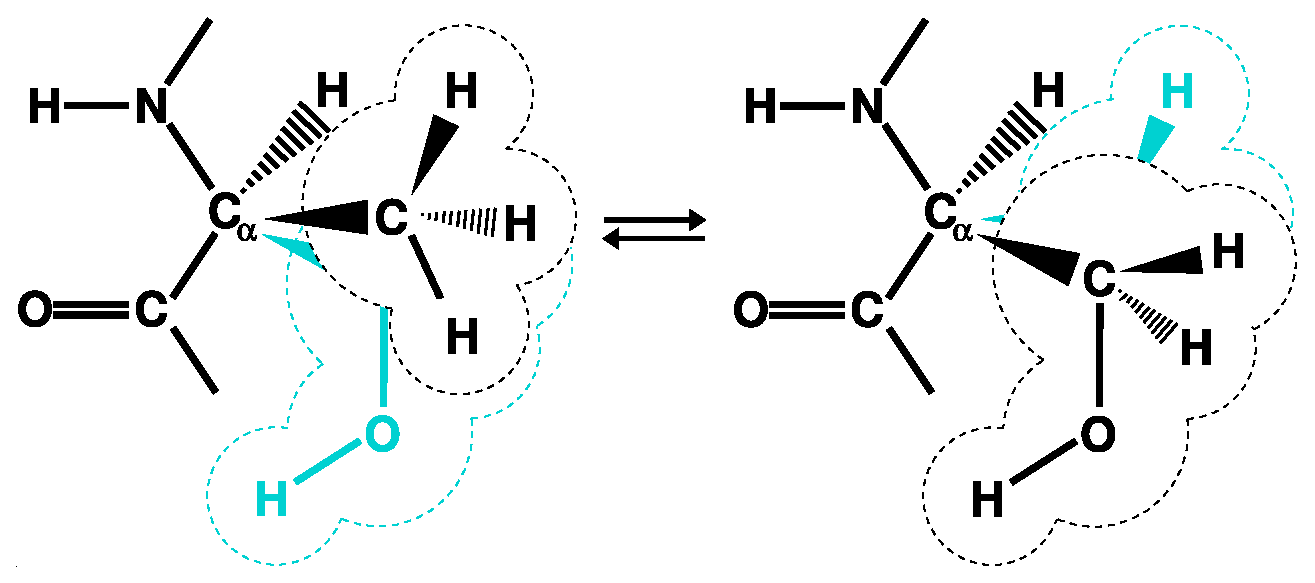
\includegraphics[width=12.5cm]{figures/dual_top}}
  \caption{Dual topology description for an alchemical simulation.
           Case example of the mutation of alanine into serine.
           The lighter color denotes the non--interacting, alternate
           state.
           \label{fig:dual_top}}
\end{figure}


The energy and forces are defined as a function of $\lambda$, in
such a fashion that the interaction of the methyl group of alanine
with the rest of the protein is effective at the beginning of the
simulation, \ie $\lambda$ = 0, while the glycine C$_\alpha$ hydrogen
atom does not interact with the rest of the protein, and {\it vice versa}
at the end of the simulation, \ie $\lambda$ = 1. For intermediate
values of $\lambda$, both the alanine and the glycine side chains
participate in non--bonded interactions with the rest of the
protein, scaled on the basis of the current value of $\lambda$. It
should be clearly understood that these side chains never
interact with each other. Construction of an appropriate
list of excluded atoms, common to the two alternate topologies,
is, therefore, necessary.


It is also worth noting that
the free energy calculation does not alter intramolecular
potentials, \eg bond stretch, valence angle deformation and torsions,
in the course of the simulation.
In calculations targeted at the estimation
of free energy differences between two states characterized by
distinct environments --- \eg a ligand, bound to a protein in
the first simulation,
and solvated in water, in the second --- as is the
case for most free energy calculations that make use of a thermodynamic
cycle, perturbation of intramolecular terms may, by and large, be safely
avoided~\cite{Boresch1999}.



\subsection{Implementation of free energy perturbation in NAMD}


The procedure implemented in NAMD is particularly
adapted for performing free
energy calculations that split the $\lambda$
reaction path into a number of non--physical,
intermediate states, or ``windows''. Separate simulations
can be started for each window.
Alternatively, the {\sc Tcl} scripting ability of
NAMD can be employed advantageously
to perform the complete simulation in a single run.
An example making use of such script is supplied at the end
of this user guide.


The following keywords can be used to control the alchemical free
energy calculations.


\begin{itemize}
\item
\NAMDCONFWDEF{fep}{ Is alchemical FEP to be performed? }
{{\tt on} or {\tt off}}
{{\tt off}} {Turns on hamiltonian scaling and ensemble
             averaging for alchemical FEP.}

\item
\NAMDCONF{lambda}{ Coupling parameter value }
{positive decimal between 0.0 and 1.0}
{The coupling parameter value determining the progress of the
perturbation. The non--bonded interactions involving the atoms vanishing
in the course of the MD simulation are scaled by (1-{\tt lambda}), while
those of the growing atoms are scaled by {\tt lambda}.}

\item
\NAMDCONF{lambda2}{Coupling parameter comparison value}
{positive decimal between 0.0 and 1.0}
{The {\tt lambda2} value corresponds to the coupling parameter to be
used for sampling in the next window.  The free energy difference
between {\tt lambda2} and {\tt lambda} is calculated.  Through simulations
at progressive values of {\tt lambda} and {\tt lambda2} the total free
energy difference may be determined.}

\item
\NAMDCONFWDEF{fepEquilSteps}{Number of equilibration steps in a window,
before data collection}
{positive integer less than {\tt numSteps} or {\tt run}}
{0}
{In each window {\tt fepEquilSteps} steps of equilibration can be
performed before ensemble averaging is initiated. The output also contains
the data gathered during equilibration and is meant for analysis of
convergence properties of the FEP calculation.}

\item
\NAMDCONFWDEF{fepFile}{{\tt pdb} file with perturbation flags}
{filename}
{coordinates}
{{\tt pdb} file to be used for indicating the FEP status for each of
the atoms pertaining to the system.
If this parameter is not declared specifically, then the
{\tt pdb} file specified by
{\tt coordinates} is utilized for this information.}

\item
\NAMDCONFWDEF{fepCol}{Column in the {\tt fepFile} that carries
                      the perturbation flag}
{X, Y, Z, O or B}
{B}
{Column of the {\tt pdb} file to use for retrieving the FEP status
of each atom, \ie a flag that indicates which atom will be perturbed
in the course of the simulation.
A value of {\tt -1} in the specified column indicates the atom will
vanish during the FEP calculation, whereas a value of {\tt 1}
indicates that the atom will grow.}

\item
\NAMDCONFWDEF{fepOutFreq}{Frequency of FEP energy output in time--steps}
{positive integer}
{5}
{Every {\tt fepOutFreq} number of MD steps, the output file
{\tt fepOutFile} is updated by dumping energies that are
used for ensemble averaging.
This variable could be set to {\tt 1} to include all the
configurations for ensemble averaging. Yet, it is recommended
to update {\tt fepOutFile}  energies at longer intervals
to avoid large files containing highly correlated data.}

\item
\NAMDCONFWDEF{fepOutFile}{FEP energy output filename}
{filename}
{\tt outfilename}
{An output file named {\tt fepOutFile}, generated by NAMD,
contains the FEP energies, dumped every {\tt fepOutFreq} steps.}

\end{itemize}



\subsection{Examples of input files for running FEP alchemical calculations}


The first example illustrates the use of {\sc Tcl} scripting for running
an alchemical transformation with the FEP feature of NAMD. In this
calculation, $\lambda$ is changed continuously from 0 to 1
by increments of $\delta \lambda$ = 0.1.


\begin{tabular}{ll}
\begin{minipage}{8cm}
\begin{verbatim}
fep             on
fepfile         ion.fep
fepCol          X
fepOutfile      ion.fepout
fepOutFreq      5
fepEquilSteps   5000

set step        0.0
set dstep       0.1

while {$step <= 1.0} {
  lambda $step
  set step [expr $step + $dstep]
  lambda2 $step
  run  10000
}
\end{verbatim}
\end{minipage}
&
\begin{minipage}{7.8cm}
Turn FEP functionality on.
\newline
File containing the information about growing/shrinking atoms
described in column {\tt X}.
\newline
Output file containing the free energy.
\newline
Frequency at which {\tt fepOutFreq} is updated.
\newline
Number of equilibration steps per $\lambda$--state.
\\[0.6cm]
Starting value of $\lambda$.
\newline
Increment of $\lambda$, \ie $\delta \lambda$.
\\[0.6cm]
{\sc Tcl} script to increment $\lambda$:
\newline
\hspace{0.4cm} (1) set {\tt lambda} value;
\newline
\hspace{0.4cm} (2) increment $\lambda$;
\newline
\hspace{0.4cm} (3) set {\tt lambda2} value;
\newline
\hspace{0.4cm} (4) run 10,000 MD steps.
\\
\end{minipage}
\end{tabular}


The user should be reminded that by setting {\tt run  10000},
10,000 MD steps will be performed, which includes the
preliminary {\tt fepEquilSteps} equilibration steps.
This means that here, the ensemble average of equation~({\ref{windows}})
will be computed  over 5,000 MD steps.


Alternatively, $\lambda$--states may be declared
explicitly, avoiding the use of {\sc Tcl} scripting:

\begin{tabular}{ll}
\begin{minipage}{8cm}
\begin{verbatim}
lambda          0.0
lambda2         0.1
run             10000
\end{verbatim}
\end{minipage}
&
\begin{minipage}{7.8cm}
(1) set {\tt lambda} value;
\newline
(2) set {\tt lambda2} value;
\newline
(3) run 10,000 MD steps.
\end{minipage}
\end{tabular}


This option is generally preferred to set up windows of diminishing
widths as $\lambda \rightarrow$ 0 or 1 --- a way to circumvent
end--point singularities caused by appearing atoms that may
clash with their surroundings. It may be used in conjunction
with a soft--core potential (see relevant section).



\subsection{Description of FEP simulation output }


The {\tt fepOutFile} contains electrostatic and van der Waals energy
data calculated for {\tt lambda} and {\tt lambda}, written every
{\tt fepOutFreq} steps. The column {\tt dE} is the energy
difference of the single configuration, {\tt dE\_avg} and {\tt dG}
are the instantaneous ensemble average of the energy and the calculated
free energy at the time step specified in column 2, respectively.
The temperature is specified in the penultimate column. Upon completion
of {\tt fepEquilSteps} steps, the calculation of {\tt dE\_avg} and
{\tt dG} is restarted. The accumulated net free energy change is written
at each lambda value and at the end of the simulation. The cumulative
average energy {\tt dE\_avg} value may be summed using the
trapezoidal rule to obtain an approximate thermodynamic integration (TI)
estimate for the free energy change during the run.


Whereas the FEP module of NAMD supplies free energy differences
determined from equation~({\ref{fep}}), the wealth of information
available in {\tt fepOutFile} may be utilized profitably to
explore different routes towards the estimation of $\Delta A$. As
commented on previously, TI may constitute one such route. The
simple overlap sampling (SOS) represents an interesting alternative,
that combines advantageously \emph{forward} and \emph{reverse}
transformations to improve convergence and accuracy of the
calculation~\cite{lu2004}. The linear scaling of the Hamiltonian
highlighted in equation~({\ref{linear}}) obviates the need for
explicit simulation of the reverse transformation, because:


\begin{equation}
{\cal H}({\bf x}, {\bf p}_x; \lambda_i) - {\cal H}({\bf x}, {\bf p}_x; \lambda_{i+1}) =
\frac{\lambda_i - \lambda_{i+1}}
     {\lambda_{i+2} - \lambda_{i+1}} \
\left[
{\cal H}({\bf x}, {\bf p}_x; \lambda_{i+2}) - {\cal H}({\bf x}, {\bf p}_x; \lambda_{i+1})
\right]
\end{equation}


The free energy difference between states $\lambda_i$ and
$\lambda_{i+1}$ may then be expressed as:


\begin{eqnarray}
\exp(-\beta \Delta A_{i \rightarrow i+1}) & = &
\frac{\displaystyle
      \left\langle \exp\left\{-\frac{\beta}{2}
                       \left[
                       {\cal H}({\bf x}, {\bf p}_x; \lambda_{i+1}) - {\cal H}({\bf x}, {\bf p}_x; \lambda_i)
                       \right]
                       \right\}
      \right\rangle_i}
      {\displaystyle
       \left\langle \exp\left\{-\frac{\beta}{2}
                       \left[
                       {\cal H}({\bf x}, {\bf p}_x; \lambda_i) - {\cal H}({\bf x}, {\bf p}_x; \lambda_{i+1})
                       \right]
                       \right\}
      \right\rangle_{i+1}}
\\
& = &
\frac{\displaystyle
      \left\langle \exp\left\{-\frac{\beta}{2}
                       \left[
                       {\cal H}({\bf x}, {\bf p}_x; \lambda_{i+1}) - {\cal H}({\bf x}, {\bf p}_x; \lambda_i)
                       \right]
                       \right\}
      \right\rangle_i}
      {\displaystyle
       \left\langle \exp\left\{-\frac{\beta}{2} \
                       \frac{\lambda_i - \lambda_{i+1}}
                            {\lambda_{i+2} - \lambda_{i+1}} \
                       \left[
                       {\cal H}({\bf x}, {\bf p}_x; \lambda_{i+2}) - {\cal H}({\bf x}, {\bf p}_x; \lambda_{i+1})
                       \right]
                       \right\}
      \right\rangle_{i+1}}
\nonumber
\label{sos}
\end{eqnarray}



%\bibliographystyle{unsrt}
%\bibliography{../../LaTeX/Bibliography/data_base}

%\end{document}
